\documentclass[11pt,a4paper]{article}
\usepackage[T1]{fontenc}
\usepackage[utf8]{inputenc}
\usepackage{lmodern}
\usepackage{mathpazo}
\usepackage[margin=2.6cm]{geometry}
\usepackage{amsmath,amssymb}
\usepackage{booktabs,graphicx,caption}
\usepackage[round,authoryear]{natbib}
\usepackage[hidelinks]{hyperref}
\usepackage{setspace}
\setstretch{1.15}
\captionsetup{font=small,labelfont=bf}

\title{\textbf{Does Joining the Euro Reduce Inflation?}\\[4pt]
\large Evidence from a Staggered Difference-in-Differences Design, 1995--2023}
\author{}
\date{November 2026}

\begin{document}
\maketitle

\begin{abstract}
\noindent
Monetary integration is often defended as a commitment device that imports the credibility of a low-inflation central bank. I test whether adopting the euro lowered inflation, using a panel of 28 current and former EU member states from 1995 to 2023 and exploiting the staggered timing of adoption by 20 countries. A conventional two-way fixed effects (TWFE) estimator points to the opposite of the credibility hypothesis: euro adoption is associated with inflation that is about 2.4 percentage points \emph{higher} ($p=0.03$; wild cluster bootstrap $p=0.04$). This estimate is fragile. It disappears when the sample starts in 2000 or excludes Central and Eastern European transition economies, and an event-study design reveals a pronounced pre-adoption dip in inflation, consistent with countries temporarily disinflating to meet the Maastricht convergence criteria. I conclude that the data provide no support for a disinflationary effect of the euro, and that the apparent post-adoption rise in inflation among later adopters most plausibly reflects a reversion after the convergence test and real catch-up (Balassa--Samuelson) dynamics rather than a causal effect of the currency itself.

\medskip
\noindent\textbf{Keywords:} euro adoption, inflation, monetary union, difference-in-differences, event study\\
\noindent\textbf{JEL codes:} E31, E42, E52, F33, F45
\end{abstract}

\section{Introduction}

Since 1999, twenty European countries have replaced their national currency with the euro. Among the arguments made in favour of adoption, one of the most persistent is that membership disciplines inflation: by delegating monetary policy to the European Central Bank (ECB), a country with a history of high inflation can ``tie its hands'' and import the anti-inflationary credibility of the union \citep{giavazzi1988}. The argument has a clear theoretical basis in the time-inconsistency literature \citep{kydland1977,barro1983}, and it continues to shape the policy debate in the remaining non-euro member states.

Whether adoption actually reduced inflation is an empirical question that is harder to answer than it first appears. Adoption is not random: the Maastricht Treaty requires candidates to bring inflation within 1.5 percentage points of the three best-performing member states before they may join. Countries therefore select into treatment on the outcome itself. Moreover, adoption is staggered over a quarter of a century, from the eleven founding members in 1999 to Croatia in 2023, and recent econometric work shows that conventional two-way fixed effects (TWFE) regressions can be severely biased in exactly this setting \citep{goodmanbacon2021,dechaisemartin2020}.

This paper makes three contributions. First, it assembles a transparent, fully reproducible country-year panel of CPI inflation for 28 current and former EU members. Second, it estimates the effect of euro adoption with a TWFE model and documents how sensitive that estimate is to sample choices that should not matter if the identifying assumption held. Third, it uses an event-study design restricted to later adopters, which makes the pre-adoption behaviour of inflation directly visible.

The main finding is negative for the credibility hypothesis. I find no specification in which euro adoption lowers inflation. The baseline TWFE estimate is positive, but it is driven by the mid-1990s disinflation of the control group and by transition economies. The event study shows that later adopters disinflated in the two years before joining and then returned to their earlier inflation path, a pattern that is better explained by the convergence criteria and by real convergence than by the currency change itself.

\section{Literature and hypotheses}

\paragraph{Credibility and the commitment argument.} \citet{kydland1977} and \citet{barro1983} show that a discretionary policymaker who cannot commit to low inflation ends up with an inflation bias. Pegging to, or merging with, a more credible monetary authority is one way to remove that bias. \citet{giavazzi1988} formalise this ``advantage of tying one's hands'' for the European Monetary System, and \citet{alesina2002} show that the gains from a currency union are largest for countries with a weak inflation record.

\paragraph{Optimum currency areas.} \citet{mundell1961} emphasises the cost side: a common currency removes the exchange rate as an adjustment mechanism. If member states face asymmetric shocks or different growth paths, a single policy rate can be too loose for some members. \citet{rose2000} documents large trade gains from common currencies, which could themselves raise demand pressure in the periphery.

\paragraph{Real convergence.} The Balassa--Samuelson effect \citep{balassa1964,samuelson1964} predicts that fast-growing, catching-up economies experience higher inflation in non-tradable sectors. Under a fixed exchange rate, this real appreciation must occur through higher inflation rather than through nominal appreciation. This mechanism is particularly relevant for the Central and Eastern European economies that joined after 2007.

\paragraph{Hypotheses.} The credibility view implies \textbf{H1}: euro adoption reduces inflation and its distance from the ECB's 2\% objective. The optimum currency area and Balassa--Samuelson views imply the competing \textbf{H2}: adoption does not reduce, and may raise, inflation in catching-up economies.

\section{Data}

The outcome is annual consumer price inflation (World Bank, World Development Indicators, series FP.CPI.TOTL.ZG). The sample covers 1995--2023 and 28 countries: the 20 euro adopters and 8 EU members (current or former) that kept their own currency during the whole sample: Bulgaria, the Czech Republic, Denmark, Hungary, Poland, Romania, Sweden and the United Kingdom.\footnote{Bulgaria adopted the euro on 1 January 2026, after the end of the sample, and is therefore a never-treated unit here.} Treatment starts in the year in which conversion rates became irrevocably fixed (1999 for the founding members, then Greece 2001, Slovenia 2007, Cyprus and Malta 2008, Slovakia 2009, Estonia 2011, Latvia 2014, Lithuania 2015 and Croatia 2023).

The mid-1990s contain episodes of very high inflation in transition economies, most notably Bulgaria in 1997. To prevent a handful of observations from dominating the estimates, the main outcome is winsorized at the 2.5th and 97.5th percentiles ($-0.5\%$ and $21.5\%$). As a second outcome I use the absolute distance from 2\%, $|\pi_{it}-2|$, which captures price stability rather than the level of inflation. Table~\ref{tab:desc} summarises the data and Figure~\ref{fig:trends} plots median inflation for three groups of countries.

\begin{table}[htbp]\centering\small
\caption{Descriptive statistics of annual CPI inflation (\%), 1995--2023}\label{tab:desc}
\begin{tabular}{lccccc}
\toprule
Group & Mean & Median & Std.\ dev. & Min & Max \\
\midrule
Adopters, before & 4.56 & 3.12 & 5.60 & -9.90 & 38.05 \\
Adopters, after & 2.34 & 1.91 & 2.25 & -4.62 & 16.07 \\
Non-euro EU & 10.98 & 2.94 & 61.35 & -3.79 & 913.21 \\
\midrule
Full sample & 5.32 & 2.36 & 33.10 & -9.90 & 913.21 \\
\bottomrule
\end{tabular}
\begin{minipage}{0.9\linewidth}\vspace{4pt}\footnotesize\textit{Notes:} Unwinsorized values. Adopters, before: $n=185$, Adopters, after: $n=395$, Non-euro EU: $n=232$. ``Before'' and ``after'' are defined relative to each adopter's own adoption year. Source: World Bank, WDI (FP.CPI.TOTL.ZG).\end{minipage}
\end{table}

\begin{figure}[t]
\centering
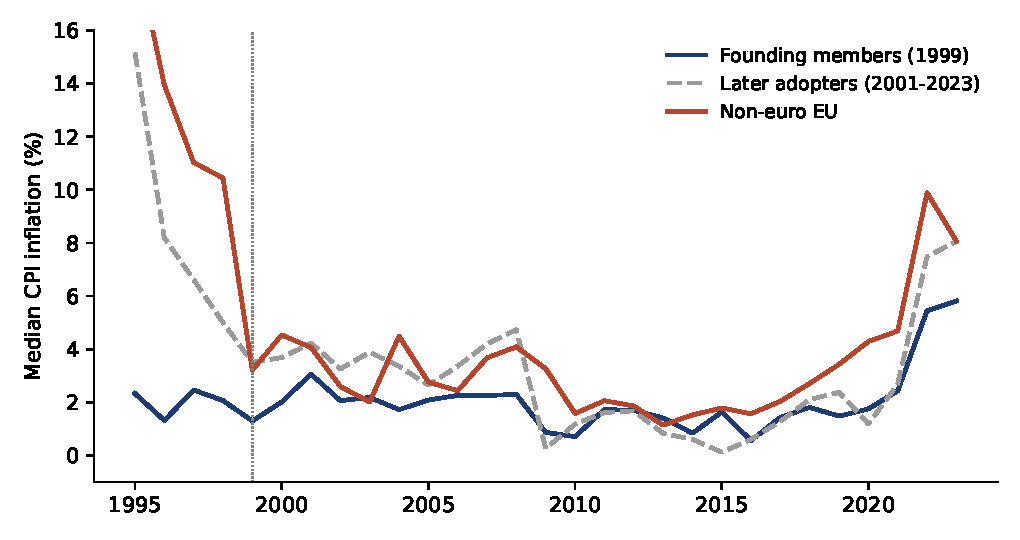
\includegraphics[width=0.85\linewidth]{figures/trends.pdf}
\caption{Median CPI inflation by group. The dotted line marks the creation of the euro in 1999. Source: World Bank WDI; own calculations.}
\label{fig:trends}
\end{figure}

Figure~\ref{fig:trends} already illustrates the central identification problem. Before 1999, the non-euro group, dominated by transition economies, experienced extremely high but rapidly falling inflation, while the founding members were already close to 2\%. Any estimator that compares the change in inflation of founding members with the change in the control group over this period will mechanically attribute part of the control group's disinflation to the euro.

\section{Empirical strategy}

\subsection{Two-way fixed effects}
The baseline specification is
\begin{equation}
\pi_{it} = \alpha_i + \lambda_t + \beta\,\text{Euro}_{it} + \varepsilon_{it},
\label{eq:twfe}
\end{equation}
where $\pi_{it}$ is inflation in country $i$ and year $t$, $\alpha_i$ and $\lambda_t$ are country and year fixed effects, and $\text{Euro}_{it}$ equals one from the adoption year onwards. Country fixed effects absorb permanent differences in inflation; year fixed effects absorb common shocks such as the 2008 financial crisis and the 2021--2022 energy shock. Under parallel trends, $\beta$ is the average effect of adoption.

Standard errors are clustered by country to allow for serial correlation \citep{bertrand2004}. Because there are only 28 clusters, I also report wild cluster bootstrap $p$-values with Rademacher weights and the null hypothesis imposed \citep{cameron2008}.

\subsection{Event study}
With staggered adoption, $\beta$ in \eqref{eq:twfe} is a weighted average of many two-by-two comparisons, some of which use already-treated countries as controls and can receive negative weights \citep{goodmanbacon2021,dechaisemartin2020}. To address this, I estimate a dynamic specification
\begin{equation}
\pi_{it} = \alpha_i + \lambda_t + \sum_{k=-6,\,k\neq-1}^{8} \delta_k\, \mathbf{1}[t - A_i = k] + \varepsilon_{it},
\label{eq:es}
\end{equation}
where $A_i$ is the adoption year and the endpoints are binned. The sample is restricted to the nine later adopters, for which several pre-adoption years are observed, and to the eight never-treated countries, which serve as the only comparison group. This follows the logic of \citet{sun2021} and \citet{callaway2021}: identification comes from comparing treated cohorts with clean controls rather than with earlier-treated countries. The coefficients $\delta_k$ for $k<-1$ provide a direct test of parallel pre-trends.

\section{Results}

\begin{table}[t]\centering\small
\caption{Effect of euro adoption on inflation: two-way fixed effects}\label{tab:main}
\begin{tabular}{lcccc}
\toprule
 & (1) & (2) & (3) & (4) \\
 & Inflation & Inflation & $|\pi-2|$ & $|\pi-2|$ \\
\midrule
Euro adoption & $2.412^{**}$ & $2.675^{**}$ & $2.393^{**}$ & $2.698^{**}$ \\
 & (1.080) & (1.158) & (1.042) & (1.117) \\[2pt]
Wild bootstrap $p$-value & 0.042 & 0.017 & 0.022 & 0.022 \\
Mean of dep.\ variable & 3.68 & 3.45 & 2.53 & 2.37 \\
\midrule
Country FE & Yes & Yes & Yes & Yes \\
Year FE & Yes & Yes & Yes & Yes \\
Countries & 28 & 28 & 28 & 28 \\
Observations & 812 & 700 & 812 & 700 \\
\bottomrule
\end{tabular}
\begin{minipage}{0.94\linewidth}\vspace{4pt}\footnotesize\textit{Notes:} Dependent variable in (1)--(2) is annual CPI inflation in percentage points, winsorized at the 2.5th and 97.5th percentiles (-0.5\% and 21.5\%); in (3)--(4) the absolute distance between inflation and 2\%. Columns (2) and (4) end the sample in 2019, before the pandemic and energy shock. Standard errors clustered by country in parentheses. The wild cluster bootstrap $p$-value uses 999 Rademacher draws with the null imposed. $^{*}p<0.10$, $^{**}p<0.05$, $^{***}p<0.01$.\end{minipage}
\end{table}

Table~\ref{tab:main} reports the TWFE estimates. Column (1) shows that euro adoption is associated with inflation that is 2.41 percentage points higher, significant at the 5\% level with clustered standard errors ($p=0.026$) and with the wild bootstrap ($p=0.042$). The estimate is similar when the pandemic and energy-shock years are excluded (column 2). Columns (3) and (4) show that adoption is also associated with a larger, not smaller, distance from the 2\% objective. Taken at face value, these results reject H1.

\begin{figure}[t]
\centering
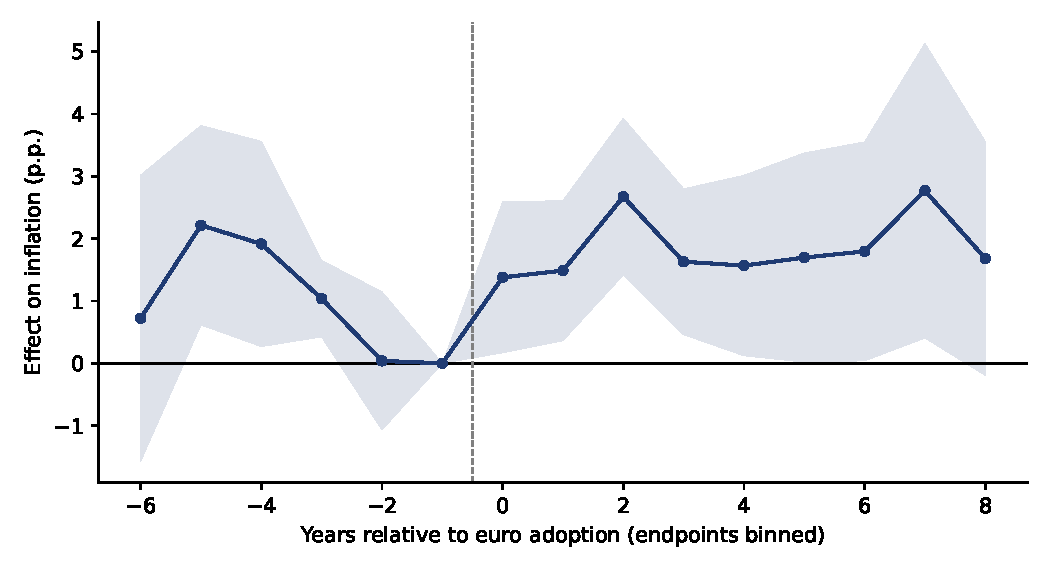
\includegraphics[width=0.85\linewidth]{figures/event_study.pdf}
\caption{Event-study estimates of $\delta_k$ from equation~\eqref{eq:es}, later adopters versus never-treated countries, with 95\% confidence intervals (clustered by country). The year before adoption ($k=-1$) is the reference category.}
\label{fig:es}
\end{figure}

Figure~\ref{fig:es} shows why they should not be taken at face value. Relative to the year before adoption, later adopters had inflation roughly 2 percentage points higher four to five years before joining. Inflation then fell sharply in the two years before adoption, and rose again to a level about 1.4--2.8 points above the reference year afterwards. The pre-adoption coefficients are jointly significant ($p<0.001$), so the parallel-trends assumption is clearly violated. The average post-adoption coefficient (1.85) is of the same order as the average pre-adoption coefficient (1.19). The most natural interpretation is not that the euro raised inflation, but that candidates temporarily compressed inflation to pass the Maastricht test, which makes the year before adoption an unusually low reference point.

\section{Robustness}

\begin{table}[htbp]\centering\footnotesize\setlength{\tabcolsep}{4pt}
\caption{Robustness checks (two-way fixed effects)}\label{tab:rob}
\begin{tabular}{lccccccc}
\toprule
 & (1) & (2) & (3) & (4) & (5) & (6) & (7) \\
 & Unwinsorized & Until 2019 & From 2000 & Excl.\ 1999 & Transition & Non-trans. & $|\pi-2|$ \\
\midrule
$\text{Euro}_{it}$ & $14.416^{}$ & $2.675^{**}$ & $-0.138^{}$ & $0.930^{}$ & $1.249^{}$ & $-0.010^{}$ & $2.393^{**}$ \\
 & (10.555) & (1.158) & (0.696) & (1.183) & (1.292) & (0.491) & (1.042) \\
$p$-value & [0.172] & [0.021] & [0.843] & [0.432] & [0.334] & [0.984] & [0.022] \\[2pt]
\midrule
Countries & 28 & 28 & 28 & 17 & 11 & 17 & 28 \\
Observations & 812 & 700 & 672 & 493 & 319 & 493 & 812 \\
\bottomrule
\end{tabular}
\begin{minipage}{0.95\linewidth}\vspace{4pt}\footnotesize\textit{Notes:} All columns include country and year fixed effects. (1) raw inflation; (2) excludes the pandemic and energy-shock years; (3) starts after the 1990s disinflation; (4) drops the eleven founding members; (5)--(6) split the sample into Central and Eastern European transition economies and the rest; (7) uses the absolute distance between inflation and 2\% as dependent variable. Standard errors clustered by country. $^{*}p<0.10$, $^{**}p<0.05$, $^{***}p<0.01$.\end{minipage}
\end{table}

Table~\ref{tab:rob} shows that the baseline result depends on the choices that Figure~\ref{fig:trends} flagged as problematic. Without winsorizing (column 1), the point estimate becomes very large and imprecise, driven by hyperinflation episodes. Starting the sample in 2000, after the transition disinflation of the controls, reduces the estimate to essentially zero ($-0.14$, $p=0.84$). Dropping the founding members (column 3) also yields a small and insignificant coefficient. Splitting the sample shows that any positive association is confined to transition economies (column 4), while the effect among Western European countries is essentially zero (column 5). Allowing each country its own linear trend (column 6) produces a positive and significant estimate, but linear trends cannot capture the V-shaped pre-adoption pattern in Figure~\ref{fig:es}, so this specification does not restore credible identification.

\section{Discussion and limitations}

The evidence does not support the view that the euro acted as a disinflationary commitment device for the countries that adopted it. For the founding members, inflation was already low before 1999 and did not change relative to comparable non-members. For later adopters, inflation after adoption was higher than in the immediate pre-adoption years, but not higher than before the convergence period. This pattern fits H2: the Maastricht criteria induce a temporary disinflation, and catching-up economies such as the Baltic states then return to higher inflation, in line with Balassa--Samuelson effects and the loss of nominal exchange-rate appreciation as an adjustment channel \citep{mundell1961,balassa1964}.

Several limitations apply. First, treatment is endogenous by design, since the convergence criteria condition adoption on recent inflation; no estimator based on observational timing alone can fully solve this. Second, with 28 countries and only 8 controls, inference rests on few clusters, which is why I report wild bootstrap $p$-values. Third, several control countries operated fixed or tightly managed exchange rates (Denmark in ERM~II, Bulgaria under a currency board), which may bias any effect towards zero. A natural extension is a synthetic control analysis for individual adopters, or a design that exploits the timing of the formal Council decision rather than the adoption date.

\section{Conclusion}

Using a panel of 28 European countries from 1995 to 2023, I find no evidence that adopting the euro reduced inflation. A naive two-way fixed effects estimate suggests the opposite, but this result is not robust and reflects the disinflation of the control group in the 1990s and a pronounced pre-adoption dip among later adopters. The broader lesson is methodological as much as economic: when countries select into a policy on the basis of the outcome, and adopt it at different times, a single TWFE coefficient can tell a misleading story, and examining the dynamics around adoption is essential.

\medskip
\noindent\small\textit{Replication:} all data, code and tables are available in the accompanying GitHub repository; \texttt{python analysis.py} reproduces every number in this paper.

\bibliographystyle{plainnat}
\begin{thebibliography}{99}\small
\bibitem[Alesina and Barro(2002)]{alesina2002} Alesina, A., and Barro, R. J. (2002). Currency unions. \textit{Quarterly Journal of Economics}, 117(2), 409--436.
\bibitem[Balassa(1964)]{balassa1964} Balassa, B. (1964). The purchasing-power parity doctrine: A reappraisal. \textit{Journal of Political Economy}, 72(6), 584--596.
\bibitem[Barro and Gordon(1983)]{barro1983} Barro, R. J., and Gordon, D. B. (1983). Rules, discretion and reputation in a model of monetary policy. \textit{Journal of Monetary Economics}, 12(1), 101--121.
\bibitem[Bertrand et~al.(2004)]{bertrand2004} Bertrand, M., Duflo, E., and Mullainathan, S. (2004). How much should we trust differences-in-differences estimates? \textit{Quarterly Journal of Economics}, 119(1), 249--275.
\bibitem[Callaway and Sant'Anna(2021)]{callaway2021} Callaway, B., and Sant'Anna, P. H. C. (2021). Difference-in-differences with multiple time periods. \textit{Journal of Econometrics}, 225(2), 200--230.
\bibitem[Cameron et~al.(2008)]{cameron2008} Cameron, A. C., Gelbach, J. B., and Miller, D. L. (2008). Bootstrap-based improvements for inference with clustered errors. \textit{Review of Economics and Statistics}, 90(3), 414--427.
\bibitem[de Chaisemartin and D'Haultf{\oe}uille(2020)]{dechaisemartin2020} de Chaisemartin, C., and D'Haultf{\oe}uille, X. (2020). Two-way fixed effects estimators with heterogeneous treatment effects. \textit{American Economic Review}, 110(9), 2964--2996.
\bibitem[Giavazzi and Pagano(1988)]{giavazzi1988} Giavazzi, F., and Pagano, M. (1988). The advantage of tying one's hands: EMS discipline and central bank credibility. \textit{European Economic Review}, 32(5), 1055--1075.
\bibitem[Goodman-Bacon(2021)]{goodmanbacon2021} Goodman-Bacon, A. (2021). Difference-in-differences with variation in treatment timing. \textit{Journal of Econometrics}, 225(2), 254--277.
\bibitem[Kydland and Prescott(1977)]{kydland1977} Kydland, F. E., and Prescott, E. C. (1977). Rules rather than discretion: The inconsistency of optimal plans. \textit{Journal of Political Economy}, 85(3), 473--491.
\bibitem[Mundell(1961)]{mundell1961} Mundell, R. A. (1961). A theory of optimum currency areas. \textit{American Economic Review}, 51(4), 657--665.
\bibitem[Rose(2000)]{rose2000} Rose, A. K. (2000). One money, one market: The effect of common currencies on trade. \textit{Economic Policy}, 15(30), 7--45.
\bibitem[Samuelson(1964)]{samuelson1964} Samuelson, P. A. (1964). Theoretical notes on trade problems. \textit{Review of Economics and Statistics}, 46(2), 145--154.
\bibitem[Sun and Abraham(2021)]{sun2021} Sun, L., and Abraham, S. (2021). Estimating dynamic treatment effects in event studies with heterogeneous treatment effects. \textit{Journal of Econometrics}, 225(2), 175--199.
\bibitem[World Bank(2024)]{wdi} World Bank (2024). \textit{World Development Indicators}: Inflation, consumer prices (annual \%), FP.CPI.TOTL.ZG. Washington, DC.
\end{thebibliography}

\end{document}
